
% =====================================================================
%  Chapter 6: Functions of Several Variables, Limits, and Continuity
%  Sections 6.1 and 6.2
% =====================================================================

\chapter{Functions of Several Variables, Limits, and Continuity}
\label{ch:6}

A curve has only one direction of travel at a time.  That made Chapter 5 feel close to
single-variable calculus: one input \(t\), one moving point \(\mathbf r(t)\), one velocity
vector \(\mathbf r'(t)\).

A surface is different.  At a point on a sheet of paper, a hillside, or a sphere, there are
many possible directions to move.  If a quantity depends on position in the plane or in
space, then one input is no longer enough.  The next few chapters begin with that
change.

\section{Functions from \texorpdfstring{\(\mathbb R^n\)}{Rn} to
\texorpdfstring{\(\mathbb R^m\)}{Rm}}
\label{sec:6.1}

Chapter 5 followed a moving point:
\[
    \mathbf r(t).
\]
The input was time, and the output was a vector.  Now the input will often be a point
in the plane or in space.  A room temperature depends on where you stand.  A pressure
inside a tank depends on position.  A wind velocity assigns an arrow to each point on a
map.

The word \emph{function} stays the same.  What changes is the shape of the input and
the shape of the output.

\subsection{A temperature field on a room floor}

Picture a rectangular room.  The floor coordinates are measured in meters, with
\[
    0\le x\le 6,
    \qquad
    0\le y\le 4.
\]
A heater sits near \((2,1)\), and a cold window runs along the north wall.  A simple
model for the temperature on the floor is
\[
    T(x,y)
    =
    20+\frac{6}{1+(x-2)^2+(y-1)^2}-\frac{y}{2}.
\]
The input is a point
\[
    (x,y)
\]
on the floor.  The output is one number,
\[
    T(x,y),
\]
the temperature in degrees Celsius.

At the heater location,
\[
    T(2,1)
    =
    20+\frac{6}{1+0+0}-\frac12
    =
    25.5.
\]
Near the far cold corner,
\[
    T(5,4)
    =
    20+\frac{6}{1+9+9}-2
    =
    18+\frac{6}{19}
    \approx 18.32.
\]

So \(T\) takes a point in the floor and returns a number.  That is a scalar-valued
function of two variables.

\begin{figure}[h]
\centering
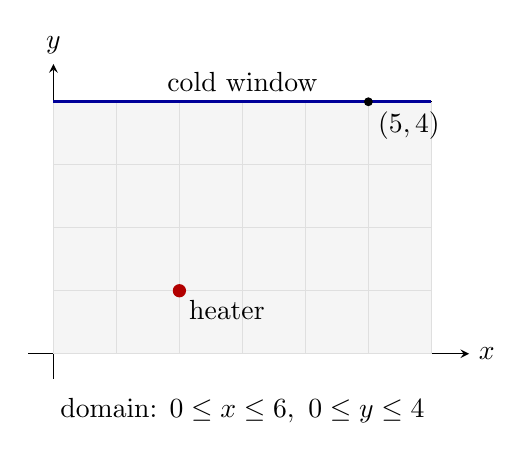
\begin{tikzpicture}[scale=0.8, >=stealth]
    \draw[fill=gray!8] (0,0) rectangle (6,4);

    \draw[->] (-0.4,0) -- (6.6,0) node[right] {\(x\)};
    \draw[->] (0,-0.4) -- (0,4.6) node[above] {\(y\)};

    \draw[step=1, gray!25, very thin] (0,0) grid (6,4);

    \fill[red!70!black] (2,1) circle (3pt);
    \node[below right] at (2,1) {heater};

    \draw[blue!60!black, very thick] (0,4) -- (6,4);
    \node[above] at (3,4) {cold window};

    \fill (5,4) circle (2pt);
    \node[below right] at (5,4) {\((5,4)\)};

    \node at (3,-0.9) {domain: \(0\le x\le 6,\ 0\le y\le 4\)};
\end{tikzpicture}
\caption{A scalar-valued function can assign one number, such as temperature, to each
point in a region.}
\end{figure}

The same input region could also carry arrows.  Suppose the air in the room slowly
circulates around a ceiling fan.  A simple two-dimensional model for the horizontal air
velocity is
\[
    \mathbf W(x,y)=\left(-\frac{y-2}{5},\frac{x-3}{5}\right).
\]
At the point \((3,0)\),
\[
    \mathbf W(3,0)=\left(\frac25,0\right),
\]
so the air is moving to the right.  At the point \((6,2)\),
\[
    \mathbf W(6,2)=\left(0,\frac35\right),
\]
so the air is moving upward.

Now the input is still a point \((x,y)\), but the output is a vector.  This is a
vector-valued function of two variables.

\begin{definition}[Function from \(\mathbb R^n\) to \(\mathbb R^m\)]
A function
\[
    F:D\subseteq \mathbb R^n\to \mathbb R^m
\]
assigns to each input
\[
    \mathbf x\in D
\]
exactly one output
\[
    F(\mathbf x)\in \mathbb R^m.
\]

The set \(D\) is called the \emph{domain}.  The set of all possible outputs is called the
\emph{range}.
\end{definition}

If \(m=1\), the output is a number.  We call the function \emph{scalar-valued}.
If \(m>1\), the output is a vector.  We call the function \emph{vector-valued}.

\begin{definition}[Scalar field and vector field]
A scalar-valued function on a region in the plane or in space is often called a
\emph{scalar field}.

A vector-valued function on a region in the plane or in space is often called a
\emph{vector field}.
\end{definition}

A temperature field is a scalar field.  A wind field is a vector field.  Later, line
integrals and surface integrals will live inside this language.

\subsection{Scalar-valued and vector-valued functions}

Here are several common shapes of functions.

\[
\begin{array}{c|c|c|c}
\text{Situation} & \text{Notation} & \text{Input} & \text{Output} \\ \hline
\text{temperature on a floor} & T(x,y) & (x,y)\in\mathbb R^2 & \text{number}\\[1mm]
\text{height of a hill} & h(x,y) & (x,y)\in\mathbb R^2 & \text{number}\\[1mm]
\text{pressure in a tank} & p(x,y,z) & (x,y,z)\in\mathbb R^3 & \text{number}\\[1mm]
\text{motion of a firefly} & \mathbf r(t) & t\in\mathbb R & \text{vector in }\mathbb R^3\\[1mm]
\text{wind on a map} & \mathbf W(x,y) & (x,y)\in\mathbb R^2 & \text{vector in }\mathbb R^2\\[1mm]
\text{surface patch} & \mathbf s(u,v) & (u,v)\in\mathbb R^2 & \text{vector in }\mathbb R^3
\end{array}
\]

The notation
\[
    F:\mathbb R^n\to\mathbb R^m
\]
does not mean that the domain must be all of \(\mathbb R^n\).  It means that the
inputs live in \(n\)-dimensional space and the outputs live in \(m\)-dimensional space.
The actual domain may be a smaller region.

For example, the temperature model above is not meant for all of \(\mathbb R^2\).
It is meant for the rectangle
\[
    D=\{(x,y):0\le x\le 6,\ 0\le y\le 4\}.
\]
Outside the room, the formula may still produce a number, but the model no longer
describes the room.

\begin{example}[A vector-valued function from Chapter 5]
The helix
\[
    \mathbf r(t)=(2\cos t,2\sin t,t)
\]
is a function
\[
    \mathbf r:\mathbb R\to\mathbb R^3.
\]
It has one input and three output components.  It is vector-valued, but it is not a
function of several variables.  The input is still one-dimensional.
\end{example}

\begin{example}[A parametrized surface]
A circular cylinder of radius \(2\) can be parametrized by
\[
    \mathbf s(\theta,z)=(2\cos\theta,2\sin\theta,z).
\]
Here
\[
    \mathbf s:\mathbb R^2\to\mathbb R^3.
\]
The input has two variables, \(\theta\) and \(z\).  The output is a point in space.

If we restrict
\[
    0\le \theta\le 2\pi,\qquad 0\le z\le 5,
\]
then the domain is a rectangle in the \((\theta,z)\)-plane, and the image is the side of
a cylinder of height \(5\).
\end{example}

The same notation covers scalar fields, vector fields, motion, and parametrized
surfaces.  The input dimension tells us how many independent variables we choose.
The output dimension tells us what kind of object the function returns.

\subsection{Domains in the plane and in space}

Sometimes a domain comes from a physical situation.  Sometimes it comes from the
formula itself.

\begin{example}[A dome over a circular floor]
A glass dome over a circular courtyard has height
\[
    h(x,y)=\sqrt{16-x^2-y^2}.
\]
The square root requires
\[
    16-x^2-y^2\ge 0.
\]
Therefore
\[
    x^2+y^2\le 16.
\]
The natural domain is the disk
\[
    D=\{(x,y):x^2+y^2\le 16\}.
\]
The formula describes the upper half of a sphere of radius \(4\).
\end{example}

\begin{example}[A formula with a missing plane]
Let
\[
    g(x,y,z)=\frac{1}{z-y}.
\]
The denominator cannot be zero, so
\[
    z-y\ne0.
\]
The domain is
\[
    D=\{(x,y,z):z\ne y\}.
\]
This is all of space except the plane
\[
    z=y.
\]
\end{example}

\begin{example}[A logarithm in space]
Let
\[
    q(x,y,z)=\ln(8-z).
\]
The logarithm requires
\[
    8-z>0,
\]
so
\[
    z<8.
\]
The domain is the open half-space below the plane \(z=8\):
\[
    D=\{(x,y,z):z<8\}.
\]
\end{example}

\begin{example}[A swirling field with a missing point]
The vector field
\[
    \mathbf V(x,y)=\frac{1}{x^2+y^2}(-y,x)
\]
is defined whenever
\[
    x^2+y^2\ne0.
\]
So its domain is
\[
    \mathbb R^2\setminus\{(0,0)\}.
\]
The origin is missing.  This small hole will matter later: fields defined on regions with
holes can behave in surprising ways.
\end{example}

The word \emph{domain} is therefore not a decoration.  It is part of the function.
Changing the domain can change the meaning of the problem.

\subsection{Examples from temperature, pressure, cost, and motion}

A function of several variables often begins as a story before it becomes a formula.

\begin{example}[Pressure in a tank]
Suppose \(z\) measures height in meters, and pressure decreases linearly as height
increases:
\[
    p(x,y,z)=120-3z.
\]
This is a scalar field in space.  It does not depend on \(x\) or \(y\), only on height.
All points with the same \(z\)-coordinate have the same pressure.
\end{example}

\begin{example}[A cost function with two inputs]
A bakery makes two kinds of loaves.  Let \(u\) be the number of sourdough loaves and
\(v\) the number of rye loaves made in one day.  A simplified cost model is
\[
    C(u,v)=400+3u+4v+0.01uv.
\]
The term \(400\) is a fixed daily cost.  The terms \(3u\) and \(4v\) are direct production
costs.  The mixed term \(0.01uv\) models the extra scheduling cost of producing both
types in the same day.

The physical domain is
\[
    u\ge0,\qquad v\ge0.
\]
Strictly speaking, \(u\) and \(v\) should be whole numbers.  Calculus treats them as
continuous variables because that approximation lets us study rates of change.
\end{example}

\begin{example}[A deformation of the plane]
A flexible sheet is pulled so that each point \((x,y)\) moves to
\[
    F(x,y)=(x+0.2y,\ y).
\]
This is a vector-valued function
\[
    F:\mathbb R^2\to\mathbb R^2.
\]
It shears the plane: points higher up move farther to the right.

This example is also a linear transformation, so it belongs to Chapter 3.  The new
point is that transformations are functions too.  They take points or vectors as inputs
and return points or vectors as outputs.
\end{example}

\subsection{Functions as fields of values}

A scalar field covers a region with numbers.  A vector field covers a region with arrows.

For example, the vector field
\[
    \mathbf W(x,y)=(-y,x)
\]
assigns an arrow to every point in the plane.  At \((1,0)\),
\[
    \mathbf W(1,0)=(0,1).
\]
At \((0,1)\),
\[
    \mathbf W(0,1)=(-1,0).
\]
The arrows circulate counterclockwise around the origin.

\begin{figure}[h]
\centering
\begin{tikzpicture}[scale=0.75, >=stealth]
    \draw[->] (-3.2,0) -- (3.4,0) node[right] {\(x\)};
    \draw[->] (0,-3.2) -- (0,3.4) node[above] {\(y\)};

    \foreach \x in {-2,-1,0,1,2} {
        \foreach \y in {-2,-1,0,1,2} {
            \pgfmathsetmacro{\u}{-0.18*\y}
            \pgfmathsetmacro{\v}{0.18*\x}
            \draw[->, thick] (\x,\y) -- ++(\u,\v);
        }
    }

    \node at (0,-4) {\(\mathbf W(x,y)=(-y,x)\)};
\end{tikzpicture}
\caption{A vector field assigns an arrow to each point.}
\end{figure}

This field will return later when we study circulation.  For now, it gives a clear
contrast:

\[
\begin{array}{c|c}
\text{scalar field} & \text{one number at each point}\\
\text{vector field} & \text{one vector at each point}
\end{array}
\]

A scalar field can be visualized in several ways.  We can make a graph, if the input is
two-dimensional.  We can draw a contour map, like a topographic map.  We can draw
level surfaces, if the input is three-dimensional.  Each picture shows the same function
from a different angle.

A formula gives exact values, but a picture tells us how those values are arranged.
That arrangement is what we look at next.

\section{Graphs, level curves, and level surfaces}
\label{sec:6.2}

Section \ref{sec:6.1} gave us scalar fields and vector fields.  Vector fields are best
drawn with arrows.  Scalar fields need a different kind of picture.

For a scalar-valued function
\[
    f(x,y),
\]
the input lives in the plane and the output is a number.  We can use the output as a
height.  That turns the function into a surface in space.

\subsection{Graphs of functions \texorpdfstring{\(z=f(x,y)\)}{z=f(x,y)}}

A market stall has a flat rectangular floor,
\[
    0\le x\le 4,\qquad 0\le y\le 3.
\]
A slanted canopy above it has height
\[
    f(x,y)=2+\frac{x}{4}+\frac{y}{6}.
\]
At the corner \((0,0)\),
\[
    f(0,0)=2.
\]
At the corner \((4,3)\),
\[
    f(4,3)=2+1+\frac12=3.5.
\]
The canopy is higher as we move in the positive \(x\)-direction and also higher as we
move in the positive \(y\)-direction.

To draw the graph, we place the point
\[
    (x,y,f(x,y))
\]
above each floor point \((x,y)\).

\begin{figure}[h]
\centering
\begin{tikzpicture}[scale=0.95, >=stealth]
    % projected floor coordinates
    \coordinate (A) at (0,0);
    \coordinate (B) at (4,0);
    \coordinate (C) at (5.35,0.75);
    \coordinate (D) at (1.35,0.75);

    % projected surface coordinates
    \coordinate (Ap) at (0,2);
    \coordinate (Bp) at (4,3);
    \coordinate (Cp) at (5.35,4.25);
    \coordinate (Dp) at (1.35,3.25);

    \draw[->] (-0.4,0) -- (6,0) node[right] {\(x\)};
    \draw[->] (0,-0.3) -- (0,4.8) node[above] {\(z\)};
    \draw[->] (0,0) -- (1.6,0.9) node[above right] {\(y\)};

    \draw[fill=gray!10] (A) -- (B) -- (C) -- (D) -- cycle;
    \draw[dashed] (A) -- (Ap);
    \draw[dashed] (B) -- (Bp);
    \draw[dashed] (C) -- (Cp);
    \draw[dashed] (D) -- (Dp);

    \draw[fill=blue!12, thick] (Ap) -- (Bp) -- (Cp) -- (Dp) -- cycle;

    \node[left] at (Ap) {\(2\)};
    \node[right] at (Cp) {\(3.5\)};
    \node at (3,4.8) {\(z=2+\dfrac{x}{4}+\dfrac{y}{6}\)};
    \node at (3,-0.8) {floor domain in the \(xy\)-plane};
\end{tikzpicture}
\caption{The graph of \(z=f(x,y)\) is made by placing height \(f(x,y)\) above each
input point \((x,y)\).}
\end{figure}

\begin{definition}[Graph of a function of two variables]
Let
\[
    f:D\subseteq\mathbb R^2\to\mathbb R.
\]
The \emph{graph} of \(f\) is the set of points in \(\mathbb R^3\)
\[
\boxed{
    \{(x,y,z): (x,y)\in D,\ z=f(x,y)\}.
}
\]
Equivalently, the graph is the surface
\[
    z=f(x,y).
\]
\end{definition}

This definition is the direct descendant of the graph of a single-variable function.
For
\[
    y=f(x),
\]
we placed the output \(y\) above the input \(x\).  Now we place the output \(z\) above
the input point \((x,y)\).

\begin{example}[A dome as a graph]
The function
\[
    h(x,y)=\sqrt{16-x^2-y^2}
\]
has domain
\[
    x^2+y^2\le 16.
\]
Its graph is
\[
    z=\sqrt{16-x^2-y^2}.
\]
Squaring gives
\[
    x^2+y^2+z^2=16,
\]
with
\[
    z\ge0.
\]
So the graph is the upper half of a sphere of radius \(4\).
\end{example}

Graphs are useful, but they have limits.  A function of three variables
\[
    f(x,y,z)
\]
would have a graph made of points
\[
    (x,y,z,f(x,y,z)).
\]
That graph lives in four-dimensional space.  We cannot draw it in the same direct way.

For scalar fields in the plane, there is another picture that is often even more useful
than the graph: the contour map.

\subsection{Contour maps and level curves}

A hiker does not need a three-dimensional plastic model of a mountain to plan a route.
A topographic map is usually better.  It joins points of equal height.

Consider a hill whose height is
\[
    H(x,y)=120-x^2-4y^2,
\]
where height is measured in meters.  The highest point is at
\[
    (0,0),
\]
where
\[
    H(0,0)=120.
\]
The set of points at height \(116\) satisfies
\[
    120-x^2-4y^2=116,
\]
so
\[
    x^2+4y^2=4.
\]
This is an ellipse.

The set of points at height \(104\) satisfies
\[
    x^2+4y^2=16.
\]
The set of points at height \(84\) satisfies
\[
    x^2+4y^2=36.
\]
Each height gives an ellipse around the summit.

\begin{figure}[h]
\centering
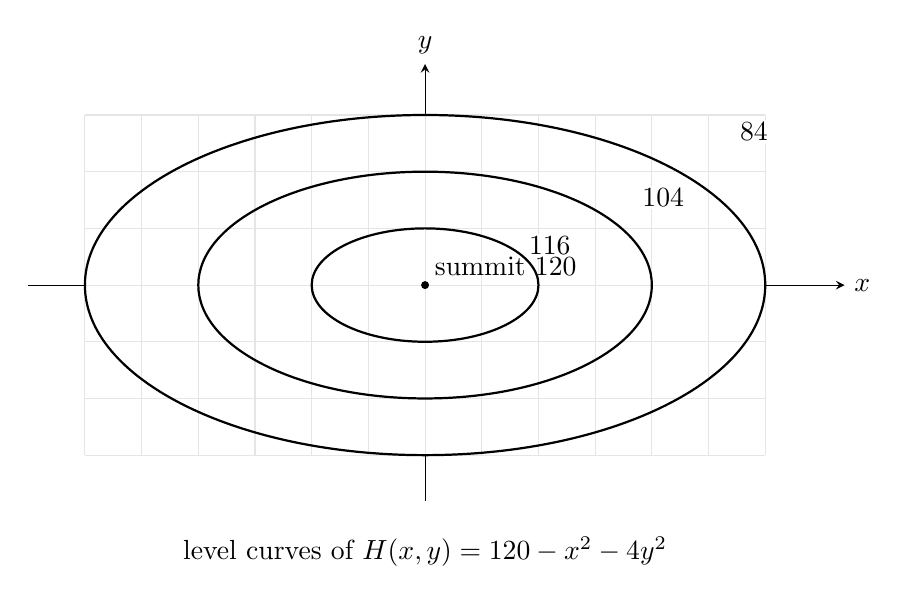
\begin{tikzpicture}[scale=0.72, >=stealth]
    \draw[->] (-7,0) -- (7.4,0) node[right] {\(x\)};
    \draw[->] (0,-3.8) -- (0,3.9) node[above] {\(y\)};

    \draw[gray!20, step=1] (-6,-3) grid (6,3);

    \draw[thick] (0,0) ellipse (2 and 1);
    \draw[thick] (0,0) ellipse (4 and 2);
    \draw[thick] (0,0) ellipse (6 and 3);

    \node[fill=white, inner sep=1pt] at (2.2,0.7) {\(116\)};
    \node[fill=white, inner sep=1pt] at (4.2,1.55) {\(104\)};
    \node[fill=white, inner sep=1pt] at (5.8,2.7) {\(84\)};

    \fill (0,0) circle (2pt);
    \node[above right] at (0,0) {summit \(120\)};

    \node at (0,-4.7) {level curves of \(H(x,y)=120-x^2-4y^2\)};
\end{tikzpicture}
\caption{Level curves of a stretched hill.  The long direction of the ellipses shows
that the hill changes more slowly east-west than north-south.}
\end{figure}

The picture tells a story.  To lose the same amount of height, you can travel farther in
the \(x\)-direction than in the \(y\)-direction.  So the hill is gentler east-west and
steeper north-south.

Now we name the idea.

\begin{definition}[Level curve]
Let
\[
    f:D\subseteq\mathbb R^2\to\mathbb R.
\]
For a constant \(c\), the \emph{level curve} of \(f\) at level \(c\) is the set
\[
\boxed{
    \{(x,y)\in D:f(x,y)=c\}.
}
\]
A contour map is a drawing of several level curves, usually labeled by their values of
\(c\).
\end{definition}

The word ``curve'' is traditional, but it comes with a warning.  A level set may be a
curve, several curves, a point, or even empty.

\begin{example}[A level curve can shrink to a point or disappear]
For
\[
    H(x,y)=120-x^2-4y^2,
\]
the level \(c=120\) gives
\[
    x^2+4y^2=0.
\]
The only solution is
\[
    (0,0).
\]
So this level set is just one point.

The level \(c=130\) gives
\[
    120-x^2-4y^2=130,
\]
or
\[
    x^2+4y^2=-10.
\]
There are no real solutions.  So this level set is empty.
\end{example}

\begin{example}[Level curves of a plane]
Let
\[
    f(x,y)=6-3x-2y.
\]
The level curve at height \(c\) is
\[
    6-3x-2y=c.
\]
Rearranging,
\[
    3x+2y=6-c.
\]
So the level curves are parallel lines.

This makes sense: the graph of \(f\) is a plane.  Slicing a tilted plane by horizontal
planes gives parallel lines.
\end{example}

\begin{example}[A saddle seen from above]
Let
\[
    S(x,y)=y^2-x^2.
\]
The level curve \(S(x,y)=0\) is
\[
    y^2-x^2=0,
\]
so
\[
    (y-x)(y+x)=0.
\]
Thus
\[
    y=x
    \qquad\text{or}\qquad
    y=-x.
\]
The zero level set is two crossing lines.

For \(c>0\), the curves
\[
    y^2-x^2=c
\]
are hyperbolas opening upward and downward.  For \(c<0\), they open left and right.
This crossing pattern is a top-down signal of a saddle surface.
\end{example}

Level curves are not merely flat drawings.  They are the shadows of horizontal slices
of the graph.

\begin{theorem}[Level curves are horizontal slices of the graph]
Let
\[
    f:D\subseteq\mathbb R^2\to\mathbb R.
\]
The intersection of the graph
\[
    z=f(x,y)
\]
with the horizontal plane
\[
    z=c
\]
is
\[
    \{(x,y,c):(x,y)\in D,\ f(x,y)=c\}.
\]
Thus it is the level curve \(f(x,y)=c\), lifted to height \(c\).
\end{theorem}

\begin{proof}
A point \((x,y,z)\) lies on the graph exactly when
\[
    z=f(x,y).
\]
It also lies in the horizontal plane \(z=c\) exactly when
\[
    z=c.
\]
Both conditions hold exactly when
\[
    f(x,y)=c
\]
and
\[
    z=c.
\]
So the intersection is the level curve \(f(x,y)=c\), placed in the plane \(z=c\).
\end{proof}

This is why a contour map can help us imagine a surface.  Draw several level curves,
then imagine each one lifted to its labeled height.

\subsection{Level surfaces}

For a function of three variables,
\[
    f(x,y,z),
\]
the graph would live in four dimensions.  But the level sets live in ordinary
three-dimensional space.

\begin{example}[Pressure levels in a tank]
Let
\[
    p(x,y,z)=120-3z.
\]
The level surface
\[
    p(x,y,z)=90
\]
satisfies
\[
    120-3z=90.
\]
So
\[
    z=10.
\]
That level surface is a horizontal plane.

More generally,
\[
    p(x,y,z)=c
\]
gives
\[
    z=\frac{120-c}{3}.
\]
So the pressure levels are horizontal planes stacked above one another.
\end{example}

\begin{definition}[Level surface]
Let
\[
    f:D\subseteq\mathbb R^3\to\mathbb R.
\]
For a constant \(c\), the \emph{level surface} of \(f\) at level \(c\) is the set
\[
\boxed{
    \{(x,y,z)\in D:f(x,y,z)=c\}.
}
\]
\end{definition}

\begin{example}[Distance from a radio beacon]
A radio beacon is located at
\[
    B=(1,-2,3).
\]
The squared distance from the beacon is
\[
    R(x,y,z)=(x-1)^2+(y+2)^2+(z-3)^2.
\]
The level surface
\[
    R(x,y,z)=9
\]
is
\[
    (x-1)^2+(y+2)^2+(z-3)^2=9.
\]
This is a sphere centered at \((1,-2,3)\) with radius \(3\).

More generally,
\[
    R(x,y,z)=c
\]
is a sphere of radius \(\sqrt c\) when \(c>0\), a single point when \(c=0\), and empty
when \(c<0\).
\end{example}

\begin{figure}[h]
\centering
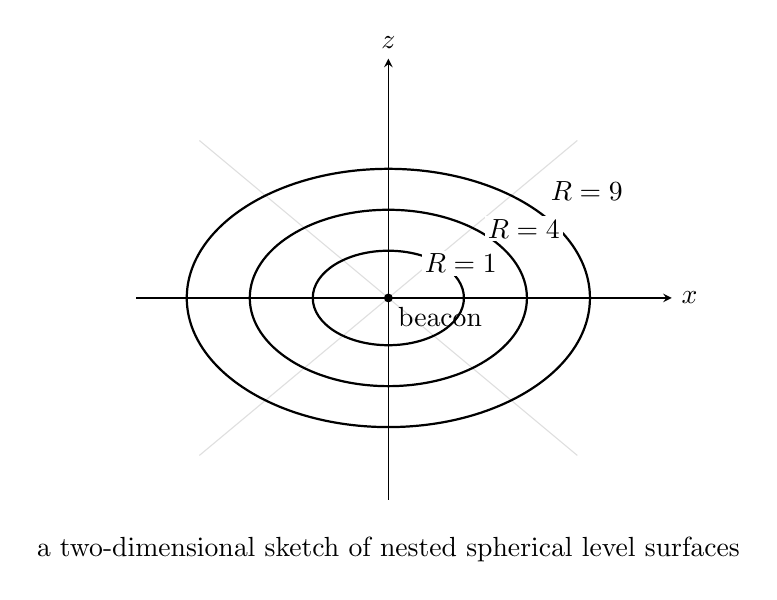
\begin{tikzpicture}[scale=0.8, >=stealth]
    \draw[->] (-4,0) -- (4.5,0) node[right] {\(x\)};
    \draw[->] (0,-3.2) -- (0,3.8) node[above] {\(z\)};

    \draw[gray!25] (-3,-2.5) -- (3,2.5);
    \draw[gray!25] (-3,2.5) -- (3,-2.5);

    \fill (0,0) circle (2pt);
    \node[below right] at (0,0) {beacon};

    \draw[thick] (0,0) ellipse (1.2 and 0.75);
    \draw[thick] (0,0) ellipse (2.2 and 1.4);
    \draw[thick] (0,0) ellipse (3.2 and 2.05);

    \node[fill=white, inner sep=1pt] at (1.15,0.55) {\(R=1\)};
    \node[fill=white, inner sep=1pt] at (2.15,1.1) {\(R=4\)};
    \node[fill=white, inner sep=1pt] at (3.15,1.7) {\(R=9\)};

    \node at (0,-4) {a two-dimensional sketch of nested spherical level surfaces};
\end{tikzpicture}
\caption{Level surfaces of squared distance are spheres centered at the source.}
\end{figure}

Level surfaces are the three-dimensional version of contour lines.  Instead of drawing
curves of equal height on a map, we draw surfaces on which a quantity stays constant.

\subsection{Reading geometry from level sets}

Level sets let us read geometry without always drawing the graph.

Here are three important habits.

First, level curves that are close together indicate rapid change.  On a topographic
map, tightly packed contour lines mean a steep slope.  Widely spaced contour lines mean
a gentle slope.

Second, the shape of a level curve tells us which directions change slowly.  For
\[
    H(x,y)=120-x^2-4y^2,
\]
the level curves are long in the \(x\)-direction and short in the \(y\)-direction.  That
means the hill changes more slowly east-west and more quickly north-south.

Third, different level curves of the same function cannot cross.  If one point lay on
both
\[
    f(x,y)=10
\]
and
\[
    f(x,y)=12,
\]
then the same input \((x,y)\) would have two outputs.  That is not a function.

The warning is that one level set can have several pieces.  For
\[
    S(x,y)=y^2-x^2,
\]
the level set \(S=0\) is the pair of lines
\[
    y=x
    \qquad\text{and}\qquad
    y=-x.
\]
Those two lines meet, but they belong to the same level value.  There is no
contradiction.

A graph, a contour map, and a formula are three ways of seeing the same scalar field.
Each has strengths.  The formula computes.  The graph shows height.  The level curves
show how height is arranged across the input region.

But pictures can also hide danger.  A surface can look calm from several straight-line
approaches to a point and still behave badly along a curved approach.  Once inputs can
approach a point from infinitely many directions, the old one-dimensional idea of a
limit needs a sharper eye.  That is the next problem.
\section{Limits in several variables}
\label{sec:6.3}

Section \ref{sec:6.2} gave us graphs, level curves, and level surfaces.  Those pictures
help us see scalar fields, but a picture is still a promise made from a distance.  Limits ask
a more delicate question:

\[
    \text{What happens as the input gets very close to one point?}
\]

In single-variable calculus, \(x\to a\) meant approaching from the left and from the right.
In the plane, a point can approach from every direction: along lines, curves, spirals,
parabolas, and paths we have not thought to name.

\subsection{Approaching a point along many paths}

Consider the function
\[
    A(x,y)=\frac{x^2-y^2}{x^2+y^2},
    \qquad (x,y)\ne(0,0).
\]
The formula is not defined at the origin.  But we can ask whether the values settle down
as \((x,y)\) approaches \((0,0)\).

Approach along the \(x\)-axis.  Then \(y=0\), so
\[
    A(x,0)=\frac{x^2}{x^2}=1
\]
for \(x\ne0\).  Along this path, the values approach
\[
    1.
\]

Approach along the \(y\)-axis.  Then \(x=0\), so
\[
    A(0,y)=\frac{-y^2}{y^2}=-1
\]
for \(y\ne0\).  Along this path, the values approach
\[
    -1.
\]

The same point gives two different limiting answers:
\[
    1
    \qquad\text{and}\qquad
    -1.
\]
So the function has no limit at the origin.

\begin{figure}[h]
\centering
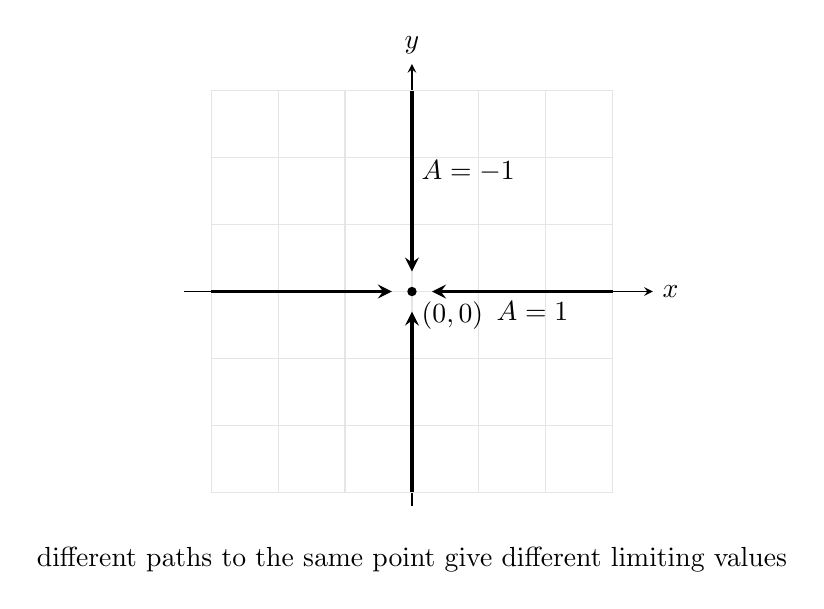
\begin{tikzpicture}[scale=0.85, >=stealth]
    \draw[->] (-3.4,0) -- (3.6,0) node[right] {\(x\)};
    \draw[->] (0,-3.2) -- (0,3.4) node[above] {\(y\)};

    \draw[gray!20, step=1] (-3,-3) grid (3,3);

    \fill (0,0) circle (2pt);
    \node[below right] at (0,0) {\((0,0)\)};

    \draw[->, very thick] (3,0) -- (0.3,0);
    \draw[->, very thick] (-3,0) -- (-0.3,0);
    \node[below] at (1.8,0) {\(A=1\)};

    \draw[->, very thick] (0,3) -- (0,0.3);
    \draw[->, very thick] (0,-3) -- (0,-0.3);
    \node[right] at (0,1.8) {\(A=-1\)};

    \node at (0,-4.0) {different paths to the same point give different limiting values};
\end{tikzpicture}
\caption{A two-variable limit must survive every possible approach to the point.}
\end{figure}

This is the main new issue.  A two-variable limit is not a left-right test.  It is an
all-paths test.

\begin{definition}[Limit of a function of two variables]
Let
\[
    f:D\subseteq\mathbb R^2\to\mathbb R.
\]
We write
\[
\boxed{
    \lim_{(x,y)\to(a,b)} f(x,y)=L
}
\]
if the values \(f(x,y)\) get arbitrarily close to \(L\) whenever \((x,y)\) is sufficiently
close to \((a,b)\), with \((x,y)\ne(a,b)\).

The point \((a,b)\) does not have to be in the domain of \(f\).  A limit is about nearby
points, not necessarily the point itself.
\end{definition}

The phrase ``whenever \((x,y)\) is sufficiently close'' means from every direction and
along every path.  If even one path gives a different answer, the limit fails.

\subsection{Path tests for nonexistence of a limit}

A path is a curve approaching the point.  If a limit exists, every path must see the same
limiting value.

The quickest way to disprove a limit is to find two paths that disagree.

\begin{example}[A family of straight paths]
Let
\[
    B(x,y)=\frac{xy}{x^2+y^2},
    \qquad (x,y)\ne(0,0).
\]
Along the \(x\)-axis,
\[
    B(x,0)=0.
\]
So along that path, the values approach \(0\).

Along the line
\[
    y=x,
\]
we get
\[
    B(x,x)=\frac{x^2}{x^2+x^2}=\frac12.
\]
So along that path, the values approach \(\frac12\).

The two path limits disagree.  Therefore
\[
    \lim_{(x,y)\to(0,0)}\frac{xy}{x^2+y^2}
\]
does not exist.
\end{example}

The same function shows something stronger.  Along the line
\[
    y=mx,
\]
we get
\[
\begin{aligned}
    B(x,mx)
    &=
    \frac{x(mx)}{x^2+(mx)^2}  \\
    &=
    \frac{mx^2}{(1+m^2)x^2} \\
    &=
    \frac{m}{1+m^2},
\end{aligned}
\]
for \(x\ne0\).  Different slopes \(m\) give different limiting values.  The origin is not
approached by one road; it is approached by infinitely many roads.

\begin{theorem}[Path test for nonexistence]
Let
\[
    f:D\subseteq\mathbb R^2\to\mathbb R.
\]
Suppose two paths
\[
    \mathbf r_1(t)\to(a,b),
    \qquad
    \mathbf r_2(t)\to(a,b)
\]
as \(t\to0\), and suppose the paths stay in the domain of \(f\) except possibly at the
endpoint.

If
\[
    \lim_{t\to0} f(\mathbf r_1(t))
\]
and
\[
    \lim_{t\to0} f(\mathbf r_2(t))
\]
exist but are different, then
\[
    \lim_{(x,y)\to(a,b)} f(x,y)
\]
does not exist.
\end{theorem}

\begin{proof}
If the two-variable limit were \(L\), then \(f(x,y)\) would approach \(L\) whenever
\((x,y)\) approaches \((a,b)\).  In particular, it would approach \(L\) along every path
to \((a,b)\).

Two different path limits would force the same limit to equal two different numbers.
That is impossible.
\end{proof}

The theorem is a tool for showing that a limit does not exist.  It is not a tool for
proving that a limit exists.

Here is the trap.

\begin{example}[All straight paths agree, but the limit still fails]
Define
\[
    C(x,y)=\frac{x^2y}{x^4+y^2},
    \qquad (x,y)\ne(0,0).
\]
First approach along a straight line
\[
    y=mx.
\]
If \(m=0\), then
\[
    C(x,0)=0.
\]
If \(m\ne0\), then
\[
\begin{aligned}
    C(x,mx)
    &=
    \frac{x^2(mx)}{x^4+m^2x^2}       \\
    &=
    \frac{mx^3}{x^2(x^2+m^2)}        \\
    &=
    \frac{mx}{x^2+m^2}.
\end{aligned}
\]
As \(x\to0\),
\[
    \frac{mx}{x^2+m^2}\to0.
\]
So every straight-line path gives the limiting value \(0\).

But now approach along the parabola
\[
    y=x^2.
\]
Then
\[
\begin{aligned}
    C(x,x^2)
    &=
    \frac{x^2(x^2)}{x^4+(x^2)^2} \\
    &=
    \frac{x^4}{2x^4}             \\
    &=
    \frac12.
\end{aligned}
\]
Along this curved path, the limiting value is \(\frac12\).

So the full limit does not exist, even though every straight-line test gave \(0\).
Straight roads are not enough.
\end{example}

The moral is important:

\[
    \text{Different path limits disprove a limit.}
\]
But
\[
    \text{matching path limits along a few paths do not prove a limit.}
\]

To prove a limit, we need a method that controls all approaches at once.

\subsection{Polar-coordinate tests near the origin}

Near the origin, polar coordinates are built for limits.  Every point near \((0,0)\) can
be written as
\[
    x=r\cos\theta,\qquad y=r\sin\theta,
\]
where
\[
    r=\sqrt{x^2+y^2}.
\]
Approaching the origin means
\[
    r\to0.
\]
The angle \(\theta\) may stay fixed, change, or spin wildly.  A good polar argument
must work no matter what \(\theta\) does.

\begin{example}[A polar-coordinate proof of a limit]
Let
\[
    D(x,y)=\frac{x^2y}{x^2+y^2},
    \qquad (x,y)\ne(0,0).
\]
We want to find
\[
    \lim_{(x,y)\to(0,0)}D(x,y).
\]

Use polar coordinates:
\[
    x=r\cos\theta,\qquad y=r\sin\theta.
\]
Then
\[
\begin{aligned}
D(x,y)
&=
\frac{(r\cos\theta)^2(r\sin\theta)}{r^2} \\
&=
r\cos^2\theta\sin\theta.
\end{aligned}
\]
Therefore
\[
    |D(x,y)|
    =
    |r\cos^2\theta\sin\theta|.
\]
Since
\[
    |\cos^2\theta\sin\theta|\le1,
\]
we get
\[
    |D(x,y)|\le r.
\]
As \((x,y)\to(0,0)\), we have \(r\to0\).  So
\[
    |D(x,y)|\le r\to0.
\]
By the squeeze idea from single-variable calculus,
\[
\boxed{
    \lim_{(x,y)\to(0,0)}\frac{x^2y}{x^2+y^2}=0.
}
\]
\end{example}

The key was not merely rewriting in polar coordinates.  The key was finding a bound
that did not depend on \(\theta\).

\begin{theorem}[Polar squeeze test near the origin]
Suppose
\[
    f(x,y)
\]
is defined near \((0,0)\), except possibly at \((0,0)\).  Write
\[
    x=r\cos\theta,\qquad y=r\sin\theta.
\]
If there is a function \(g(r)\) such that
\[
    |f(r\cos\theta,r\sin\theta)-L|\le g(r)
\]
for all sufficiently small \(r>0\) and all angles \(\theta\), and if
\[
    \lim_{r\to0^+}g(r)=0,
\]
then
\[
\boxed{
    \lim_{(x,y)\to(0,0)}f(x,y)=L.
}
\]
\end{theorem}

\begin{proof}
The distance from \((x,y)\) to the origin is \(r\).  As \((x,y)\to(0,0)\), we have
\(r\to0^+\).  The inequality
\[
    |f(r\cos\theta,r\sin\theta)-L|\le g(r)
\]
holds for every angle, so it controls every possible approach to the origin.  Since
\(g(r)\to0\), the difference
\[
    |f(x,y)-L|
\]
must also go to \(0\).
\end{proof}

The phrase ``for all angles \(\theta\)'' is the heart of the theorem.  Without it, a path
could hide in the angle dependence.

\begin{example}[Polar coordinates can also reveal failure]
Return to
\[
    A(x,y)=\frac{x^2-y^2}{x^2+y^2}.
\]
In polar coordinates,
\[
\begin{aligned}
    A(x,y)
    &=
    \frac{r^2\cos^2\theta-r^2\sin^2\theta}{r^2} \\
    &=
    \cos^2\theta-\sin^2\theta \\
    &=
    \cos(2\theta).
\end{aligned}
\]
The expression does not depend on \(r\) at all.  It depends only on the angle.

Along \(\theta=0\),
\[
    A=1.
\]
Along \(\theta=\frac{\pi}{2}\),
\[
    A=-1.
\]
No matter how close we get to the origin, the angle still controls the value.  So the
limit does not exist.
\end{example}

To use polar coordinates near another point \((a,b)\), shift the point to the origin:
\[
    u=x-a,\qquad v=y-b.
\]
Then write
\[
    u=r\cos\theta,\qquad v=r\sin\theta.
\]
Approaching \((a,b)\) is the same as
\[
    r=\sqrt{(x-a)^2+(y-b)^2}\to0.
\]

\subsection{The formal limit definition in \texorpdfstring{\(\mathbb R^n\)}{Rn}}

The words ``nearby inputs give nearby outputs'' are right, but sometimes we need the
exact sentence behind them.

For a function
\[
    F:D\subseteq\mathbb R^n\to\mathbb R^m,
\]
both the input and the output may be vectors.  Distance measures closeness in both
spaces.

\begin{definition}[Formal limit in \(\mathbb R^n\)]
Let
\[
    F:D\subseteq\mathbb R^n\to\mathbb R^m.
\]
We write
\[
\boxed{
    \lim_{\mathbf x\to\mathbf a}F(\mathbf x)=\mathbf L
}
\]
if the following condition holds:

For every \(\varepsilon>0\), there is a \(\delta>0\) such that whenever
\[
    0<\|\mathbf x-\mathbf a\|<\delta
\]
and
\[
    \mathbf x\in D,
\]
we have
\[
    \|F(\mathbf x)-\mathbf L\|<\varepsilon.
\]
\end{definition}

This definition is just the precise version of the all-paths idea.  The condition
\[
    0<\|\mathbf x-\mathbf a\|<\delta
\]
says that the input is close to \(\mathbf a\), but not equal to \(\mathbf a\).  The condition
\[
    \|F(\mathbf x)-\mathbf L\|<\varepsilon
\]
says that the output is close to \(\mathbf L\).

\begin{example}[A direct limit proof for a linear function]
Let
\[
    f(x,y)=3x-2y.
\]
We claim that
\[
    \lim_{(x,y)\to(1,4)} f(x,y)=f(1,4)=-5.
\]
Compute the difference:
\[
\begin{aligned}
    |f(x,y)-(-5)|
    &=
    |3x-2y+5|  \\
    &=
    |3(x-1)-2(y-4)|.
\end{aligned}
\]
Using the triangle inequality,
\[
    |3(x-1)-2(y-4)|
    \le
    3|x-1|+2|y-4|.
\]
Also,
\[
    |x-1|\le \sqrt{(x-1)^2+(y-4)^2},
\]
and
\[
    |y-4|\le \sqrt{(x-1)^2+(y-4)^2}.
\]
Therefore
\[
\begin{aligned}
    |f(x,y)-(-5)|
    &\le
    5\sqrt{(x-1)^2+(y-4)^2}.
\end{aligned}
\]
If
\[
    \sqrt{(x-1)^2+(y-4)^2}<\delta,
\]
then
\[
    |f(x,y)-(-5)|<5\delta.
\]
To make this less than \(\varepsilon\), choose
\[
    \delta=\frac{\varepsilon}{5}.
\]
So the formal definition confirms what geometry already suggested: a linear function
has no sudden behavior.  Its values move continuously with its inputs.
\end{example}

Vector-valued limits work component by component, just as they did for the
one-variable vector-valued functions in Chapter \ref{ch:5}.

\begin{theorem}[Componentwise limits]
Let
\[
    F:D\subseteq\mathbb R^n\to\mathbb R^m
\]
be written in components as
\[
    F(\mathbf x)=
    \bigl(F_1(\mathbf x),F_2(\mathbf x),\ldots,F_m(\mathbf x)\bigr).
\]
Let
\[
    \mathbf L=(L_1,L_2,\ldots,L_m).
\]
Then
\[
    \lim_{\mathbf x\to\mathbf a}F(\mathbf x)=\mathbf L
\]
if and only if
\[
    \lim_{\mathbf x\to\mathbf a}F_i(\mathbf x)=L_i
\]
for every component \(i=1,2,\ldots,m\).
\end{theorem}

\begin{proof}
If the vector \(F(\mathbf x)\) approaches \(\mathbf L\), then the distance between them
goes to \(0\).  Each component difference is no larger in absolute value than that
distance, so each component approaches its limiting value.

Conversely, if each component difference approaches \(0\), then
\[
    \|F(\mathbf x)-\mathbf L\|
    =
    \sqrt{
    (F_1(\mathbf x)-L_1)^2+\cdots+(F_m(\mathbf x)-L_m)^2
    }
\]
also approaches \(0\).  So the vector limit holds.
\end{proof}

\begin{example}[A vector-valued limit]
Let
\[
    F(x,y)=
    \left(
        x+y,\;
        \frac{x^2y}{x^2+y^2}
    \right),
    \qquad (x,y)\ne(0,0).
\]
As \((x,y)\to(0,0)\),
\[
    x+y\to0.
\]
From the polar-coordinate example above,
\[
    \frac{x^2y}{x^2+y^2}\to0.
\]
Therefore
\[
    \lim_{(x,y)\to(0,0)}F(x,y)=(0,0).
\]
\end{example}

A limit does not care what happens at the point itself.  That is both useful and a little
dangerous.

For example, define
\[
    G(x,y)=
    \begin{cases}
    \dfrac{x^2y}{x^2+y^2}, & (x,y)\ne(0,0),\\[2mm]
    17, & (x,y)=(0,0).
    \end{cases}
\]
The limit at the origin is still
\[
    0.
\]
But the actual value at the origin is
\[
    17.
\]
So the surface has a perfectly good limiting height, but the function has placed the
point at the wrong height.

That mismatch is exactly what continuity is designed to catch.  A limit asks what the
nearby values want the answer to be.  Continuity asks whether the function actually
listens.

\section{Continuity}
\label{sec:6.4}

Section \ref{sec:6.3} ended with a mismatch.  The nearby values of
\[
    \frac{x^2y}{x^2+y^2}
\]
wanted to approach \(0\) at the origin, but we could still define the value at the
origin to be \(17\).  Limits notice what happens nearby.  Continuity asks whether the
function agrees with its own nearby behavior.

\subsection{Continuity as nearby inputs give nearby outputs}

A temperature field should not usually jump suddenly.  If you move a few centimeters
across a room, the temperature should change only a little.  A formula can express that
kind of steadiness.

Consider
\[
    R(x,y)=
    \begin{cases}
    \dfrac{x^2y}{x^2+y^2}, & (x,y)\ne(0,0),\\[2mm]
    0, & (x,y)=(0,0).
    \end{cases}
\]
In Section \ref{sec:6.3}, polar coordinates gave
\[
    \frac{x^2y}{x^2+y^2}
    =
    r\cos^2\theta\sin\theta.
\]
Since
\[
    \left|r\cos^2\theta\sin\theta\right|\le r,
\]
we get
\[
    \lim_{(x,y)\to(0,0)}\frac{x^2y}{x^2+y^2}=0.
\]
But now the value at the origin is also
\[
    R(0,0)=0.
\]
So
\[
    \lim_{(x,y)\to(0,0)}R(x,y)=R(0,0).
\]
There is no hole, no jump, and no mismatch.  The function is continuous at the origin.

Now change only one line:
\[
    G(x,y)=
    \begin{cases}
    \dfrac{x^2y}{x^2+y^2}, & (x,y)\ne(0,0),\\[2mm]
    17, & (x,y)=(0,0).
    \end{cases}
\]
The nearby values still approach \(0\), but the actual value is \(17\).  Therefore
\[
    \lim_{(x,y)\to(0,0)}G(x,y)\ne G(0,0).
\]
The function is not continuous at the origin.

\begin{definition}[Continuity at a point]
Let
\[
    F:D\subseteq \mathbb R^n\to\mathbb R^m.
\]
We say that \(F\) is \emph{continuous at \(\mathbf a\in D\)} if
\[
\boxed{
    \lim_{\mathbf x\to\mathbf a}F(\mathbf x)=F(\mathbf a).
}
\]
We say that \(F\) is \emph{continuous on \(D\)} if it is continuous at every point of
\(D\).
\end{definition}

The definition contains three requirements at once:

\[
\begin{array}{ll}
\text{1.} & F(\mathbf a)\text{ must be defined.}\\[1mm]
\text{2.} & \displaystyle \lim_{\mathbf x\to\mathbf a}F(\mathbf x)\text{ must exist.}\\[3mm]
\text{3.} & \displaystyle \lim_{\mathbf x\to\mathbf a}F(\mathbf x)\text{ must equal }F(\mathbf a).
\end{array}
\]

If any one of these fails, continuity fails.

\begin{example}[A removable discontinuity]
Define
\[
    f(x,y)=\frac{x^2+y^2}{\sqrt{x^2+y^2}},
    \qquad (x,y)\ne(0,0).
\]
For \((x,y)\ne(0,0)\),
\[
    f(x,y)=\sqrt{x^2+y^2}.
\]
Thus
\[
    \lim_{(x,y)\to(0,0)} f(x,y)=0.
\]
But the original formula is not defined at \((0,0)\).  So \(f\) is not continuous at
the origin.

If we define
\[
    f(0,0)=0,
\]
then the repaired function becomes continuous at the origin.  The discontinuity was
only a missing value.
\end{example}

\begin{example}[A discontinuity that cannot be repaired]
Let
\[
    h(x,y)=\frac{xy}{x^2+y^2},
    \qquad (x,y)\ne(0,0).
\]
Along the \(x\)-axis,
\[
    h(x,0)=0.
\]
Along the line \(y=x\),
\[
    h(x,x)=\frac{x^2}{2x^2}=\frac12.
\]
The limit at the origin does not exist.  No choice of \(h(0,0)\) can make the function
continuous there.

A missing value can be repaired only when the limit exists.
\end{example}

For vector-valued functions, continuity is componentwise, just as limits are.

\begin{theorem}[Componentwise continuity]
Let
\[
    F:D\subseteq\mathbb R^n\to\mathbb R^m
\]
be written as
\[
    F(\mathbf x)=
    \bigl(F_1(\mathbf x),F_2(\mathbf x),\ldots,F_m(\mathbf x)\bigr).
\]
Then \(F\) is continuous at \(\mathbf a\) if and only if each component function
\[
    F_i:D\to\mathbb R
\]
is continuous at \(\mathbf a\).
\end{theorem}

\begin{proof}
This follows directly from the componentwise limit theorem in Section \ref{sec:6.3}.
The vector limit
\[
    \lim_{\mathbf x\to\mathbf a}F(\mathbf x)=F(\mathbf a)
\]
holds exactly when every component limit satisfies
\[
    \lim_{\mathbf x\to\mathbf a}F_i(\mathbf x)=F_i(\mathbf a).
\]
\end{proof}

\begin{example}[A continuous vector field]
The swirling field
\[
    \mathbf W(x,y)=(-y,x)
\]
is continuous everywhere in the plane.  Its components
\[
    -y
    \qquad\text{and}\qquad
    x
\]
are continuous functions.

The field
\[
    \mathbf V(x,y)=\frac{1}{x^2+y^2}(-y,x)
\]
is continuous on its domain
\[
    \mathbb R^2\setminus\{(0,0)\}.
\]
It is not continuous at the origin because it is not even defined there.  The missing
point is not a small detail; it will matter later when we study circulation around holes.
\end{example}

\subsection{Algebra of continuous functions}

Most continuous functions are built from simpler continuous functions.

For example, suppose the pressure in a tank is modeled by
\[
    p(x,y,z)=\frac{100+2z}{1+x^2+y^2}.
\]
The numerator
\[
    100+2z
\]
is continuous.  The denominator
\[
    1+x^2+y^2
\]
is continuous and never equals \(0\).  So the quotient behaves continuously everywhere
in space.

This example is so common that we turn it into a theorem.

\begin{theorem}[Algebra of continuous functions]
Suppose
\[
    f,g:D\subseteq\mathbb R^n\to\mathbb R
\]
are continuous at \(\mathbf a\in D\), and let \(c\) be a constant.  Then the following
functions are continuous at \(\mathbf a\):
\[
    f+g,\qquad f-g,\qquad cf,\qquad fg.
\]
If
\[
    g(\mathbf a)\ne0,
\]
then
\[
    \frac{f}{g}
\]
is also continuous at \(\mathbf a\).
\end{theorem}

\begin{proof}
The limit laws from Section \ref{sec:6.3} give
\[
    \lim_{\mathbf x\to\mathbf a}(f+g)(\mathbf x)
    =
    f(\mathbf a)+g(\mathbf a),
\]
and similarly for differences, constant multiples, and products.

For quotients, the limit law for quotients applies when the limiting denominator is not
zero:
\[
    \lim_{\mathbf x\to\mathbf a}g(\mathbf x)=g(\mathbf a)\ne0.
\]
Thus
\[
    \lim_{\mathbf x\to\mathbf a}\frac{f(\mathbf x)}{g(\mathbf x)}
    =
    \frac{f(\mathbf a)}{g(\mathbf a)}.
\]
\end{proof}

We required
\[
    g(\mathbf a)\ne0
\]
for a reason.

\begin{example}[Why the denominator condition matters]
Let
\[
    f(x,y)=1,
    \qquad
    g(x,y)=x^2+y^2.
\]
Both functions are continuous everywhere.  But
\[
    \frac{f(x,y)}{g(x,y)}
    =
    \frac{1}{x^2+y^2}
\]
is not continuous at the origin.  It is not even defined there, and its values become
unbounded as \((x,y)\to(0,0)\).

So a quotient of continuous functions is continuous only where the denominator is not
zero.
\end{example}

\begin{example}[A formula continuous on its natural domain]
The function
\[
    q(x,y)=\frac{\sqrt{4-x^2-y^2}}{1+xy}
\]
is continuous wherever the formula makes sense and the denominator is not zero.

The square root requires
\[
    4-x^2-y^2\ge0,
\]
so
\[
    x^2+y^2\le4.
\]
The denominator requires
\[
    1+xy\ne0.
\]
Therefore \(q\) is continuous on
\[
    \{(x,y):x^2+y^2\le4,\ xy\ne -1\}.
\]
\end{example}

This gives a practical habit:

\[
    \text{A formula made from continuous pieces is continuous wherever it is allowed to be.}
\]

The suspicious points are the places where the formula is not allowed: zero denominators,
square roots of negative numbers, logarithms of nonpositive numbers, and special
piecewise definitions.

\subsection{Continuity of compositions}

A function can feed into another function.

For example, the height of a dome over a circular floor is
\[
    h(x,y)=\sqrt{16-x^2-y^2}.
\]
In polar coordinates,
\[
    x=r\cos\theta,\qquad y=r\sin\theta.
\]
Substituting gives
\[
\begin{aligned}
    h(r\cos\theta,r\sin\theta)
    &=
    \sqrt{16-r^2\cos^2\theta-r^2\sin^2\theta}\\
    &=
    \sqrt{16-r^2}.
\end{aligned}
\]
The coordinate map
\[
    \Phi(r,\theta)=(r\cos\theta,r\sin\theta)
\]
is continuous.  The height function \(h\) is continuous on its disk.  Their composition
\[
    h\circ \Phi
\]
is continuous wherever
\[
    16-r^2\ge0.
\]

\begin{theorem}[Continuity of compositions]
Let
\[
    F:D\subseteq\mathbb R^n\to\mathbb R^m
\]
be continuous at \(\mathbf a\), and let
\[
    G:E\subseteq\mathbb R^m\to\mathbb R^k
\]
be continuous at \(F(\mathbf a)\).  If
\[
    F(D)\subseteq E,
\]
then the composition
\[
    G\circ F
\]
is continuous at \(\mathbf a\).
\end{theorem}

\begin{proof}
Since \(F\) is continuous at \(\mathbf a\),
\[
    F(\mathbf x)\to F(\mathbf a)
    \qquad\text{as}\qquad
    \mathbf x\to\mathbf a.
\]
Since \(G\) is continuous at \(F(\mathbf a)\),
\[
    G(\mathbf y)\to G(F(\mathbf a))
    \qquad\text{as}\qquad
    \mathbf y\to F(\mathbf a).
\]
Taking
\[
    \mathbf y=F(\mathbf x),
\]
we get
\[
    G(F(\mathbf x))\to G(F(\mathbf a)).
\]
So \(G\circ F\) is continuous at \(\mathbf a\).
\end{proof}

The continuity hypotheses are real.  If either piece has a jump in the wrong place,
the composition can have a jump.

\begin{example}[A discontinuous outer function can break the composition]
Let
\[
    F(x,y)=x^2+y^2,
\]
which is continuous everywhere.  Define
\[
    G(u)=
    \begin{cases}
    0, & u=0,\\
    1, & u>0.
    \end{cases}
\]
Then \(G\) is not continuous at \(u=0\).

The composition is
\[
    (G\circ F)(x,y)=
    \begin{cases}
    0, & (x,y)=(0,0),\\
    1, & (x,y)\ne(0,0).
    \end{cases}
\]
As \((x,y)\to(0,0)\), the values are always \(1\) except at the origin itself.  The
limit is \(1\), but the value at the origin is \(0\).  So the composition is not continuous
at the origin.
\end{example}

\begin{example}[A discontinuous inner function can also break the composition]
Let
\[
    F(x,y)=
    \begin{cases}
    0, & x^2+y^2<1,\\
    1, & x^2+y^2\ge1.
    \end{cases}
\]
This function jumps on the circle
\[
    x^2+y^2=1.
\]
Let
\[
    G(u)=u.
\]
The outer function \(G\) is continuous everywhere, but
\[
    G\circ F=F.
\]
So the composition is still discontinuous on the circle.  A continuous outer function
does not repair a discontinuous inner function.
\end{example}

\subsection{Continuous functions on closed and bounded regions}

Single-variable calculus has a comforting theorem: a continuous function on a closed
interval
\[
    [a,b]
\]
has a maximum and a minimum.  Multivariable calculus has the same idea, but the
interval becomes a closed and bounded region.

First, an example.

Let
\[
    H(x,y)=120-x^2-4y^2
\]
on the rectangle
\[
    D=\{(x,y):0\le x\le3,\ 0\le y\le2\}.
\]
This is the height function from our contour-map hill, restricted to a rectangular park.

The function is largest at
\[
    (0,0),
\]
where
\[
    H(0,0)=120.
\]
It is smallest at
\[
    (3,2),
\]
where
\[
    H(3,2)=120-9-16=95.
\]
So this hill has both a highest point and a lowest point on the park.

The rectangle matters.  It contains its edges, and it does not stretch to infinity.

\begin{definition}[Bounded region]
A set \(D\subseteq\mathbb R^n\) is \emph{bounded} if it fits inside some large ball.
That is, there is a number \(M\) such that
\[
    \|\mathbf x\|\le M
\]
for every \(\mathbf x\in D\).
\end{definition}

\begin{definition}[Closed region]
A set \(D\subseteq\mathbb R^n\) is \emph{closed} if it contains all of its boundary
points.

In this book, the most important examples are regions described by non-strict
inequalities, such as
\[
    x^2+y^2\le 9
\]
or
\[
    0\le x\le 3,\qquad 0\le y\le 2.
\]
\end{definition}

The disk
\[
    x^2+y^2\le1
\]
is closed and bounded.  The open disk
\[
    x^2+y^2<1
\]
is bounded but not closed, because it leaves out its boundary circle.  The whole plane
\[
    \mathbb R^2
\]
is closed but not bounded.

\begin{theorem}[Extreme Value Theorem in several variables]
Let
\[
    f:D\subseteq\mathbb R^n\to\mathbb R
\]
be continuous.  If \(D\) is closed and bounded, then \(f\) attains an absolute maximum
and an absolute minimum on \(D\).

That means there are points
\[
    \mathbf p,\mathbf q\in D
\]
such that
\[
    f(\mathbf p)\le f(\mathbf x)\le f(\mathbf q)
\]
for every \(\mathbf x\in D\).
\end{theorem}

\begin{proof}[Idea of the proof]
A closed and bounded region has no missing edge point and no escape to infinity.
A continuous function cannot jump over a value or shoot upward without nearby values
following it.  These two facts together force the highest and lowest values to be
reached.

The full proof belongs to a later analysis course.  For this course, the theorem is a
tool: on a closed and bounded region, a continuous function cannot merely approach
its maximum or minimum.  It must attain them.
\end{proof}

Each hypothesis matters.

\begin{example}[Why boundedness matters]
The function
\[
    f(x,y)=x
\]
is continuous on all of \(\mathbb R^2\).  The domain \(\mathbb R^2\) is closed, but it is
not bounded.

There is no maximum, because \(x\) can be made as large as we like.  There is no
minimum, because \(x\) can be made as negative as we like.
\end{example}

\begin{example}[Why closedness matters]
The function
\[
    f(x,y)=x^2+y^2
\]
is continuous on the open disk
\[
    D=\{(x,y):x^2+y^2<1\}.
\]
The domain is bounded, but it is not closed.

The values satisfy
\[
    0\le f(x,y)<1.
\]
The function has a minimum at \((0,0)\), but it has no maximum.  The value \(1\)
is approached near the boundary circle, but the boundary circle is not included.
\end{example}

\begin{example}[Why continuity matters]
Define
\[
    u(x,y)=
    \begin{cases}
    \dfrac{1}{x^2+y^2}, & (x,y)\ne(0,0),\\[2mm]
    0, & (x,y)=(0,0).
    \end{cases}
\]
Let
\[
    D=\{(x,y):x^2+y^2\le1\}.
\]
The domain \(D\) is closed and bounded.  But \(u\) is not continuous at the origin.

As \((x,y)\to(0,0)\), the values
\[
    \frac{1}{x^2+y^2}
\]
become arbitrarily large.  So \(u\) has no maximum on \(D\).  Closed and bounded
domains do not protect us from discontinuities.
\end{example}

Continuity is a powerful promise, but it is also easy to assume too quickly.  A formula
may look harmless from a few straight paths and still hide a thin ridge, a missing point,
or a sudden jump.  Before we move on to slopes in many directions, it is worth collecting
the main traps in one place.

\section{Warning examples}
\label{sec:6.5}

Limits and continuity in several variables have one central difficulty: there are too many
ways to approach a point.  The examples in this section are not rare tricks.  They are
the warning signs that tell us how to think.

\subsection{A function with different limits along different paths}

Let
\[
    A(x,y)=\frac{x^2-y^2}{x^2+y^2},
    \qquad (x,y)\ne(0,0).
\]
Along the \(x\)-axis,
\[
    A(x,0)=1.
\]
Along the \(y\)-axis,
\[
    A(0,y)=-1.
\]
So
\[
    \lim_{x\to0}A(x,0)=1
\]
but
\[
    \lim_{y\to0}A(0,y)=-1.
\]
The two paths disagree.  Therefore
\[
    \lim_{(x,y)\to(0,0)}A(x,y)
\]
does not exist.

In polar coordinates,
\[
    A(r\cos\theta,r\sin\theta)
    =
    \frac{r^2\cos^2\theta-r^2\sin^2\theta}{r^2}
    =
    \cos(2\theta).
\]
The value depends only on the angle.  Getting closer to the origin does not force the
function toward one number.

\begin{figure}[h]
\centering
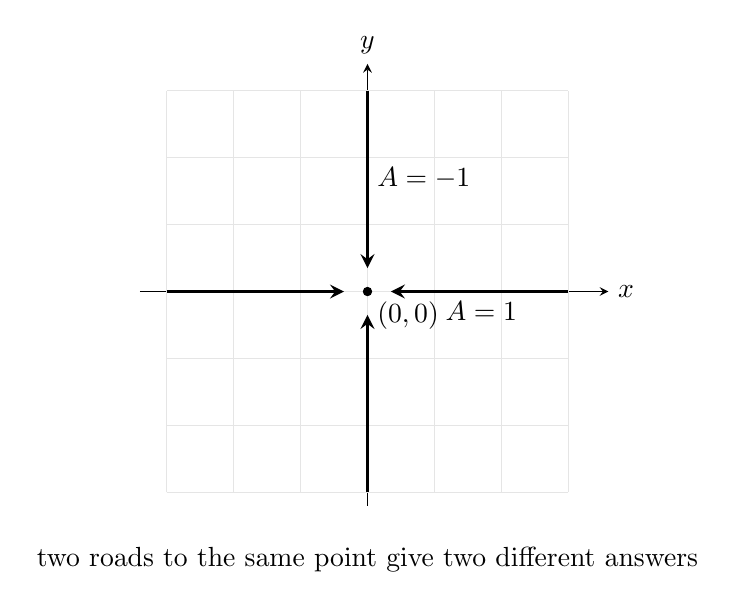
\begin{tikzpicture}[scale=0.85, >=stealth]
    \draw[->] (-3.4,0) -- (3.6,0) node[right] {\(x\)};
    \draw[->] (0,-3.2) -- (0,3.4) node[above] {\(y\)};

    \draw[gray!20, step=1] (-3,-3) grid (3,3);

    \fill (0,0) circle (2pt);
    \node[below right] at (0,0) {\((0,0)\)};

    \draw[->, very thick] (3,0) -- (0.35,0);
    \draw[->, very thick] (-3,0) -- (-0.35,0);
    \node[below] at (1.7,0) {\(A=1\)};

    \draw[->, very thick] (0,3) -- (0,0.35);
    \draw[->, very thick] (0,-3) -- (0,-0.35);
    \node[right] at (0,1.7) {\(A=-1\)};

    \node at (0,-4.0) {two roads to the same point give two different answers};
\end{tikzpicture}
\caption{Different path limits disprove a two-variable limit.}
\end{figure}

The moral is simple:

\[
    \text{One disagreement is enough to destroy a limit.}
\]

\subsection{A function whose path limits agree along lines but whose limit still fails}

Now comes the more dangerous trap.  Sometimes every straight-line test gives the same
answer, but the full limit still fails.

Let
\[
    C(x,y)=\frac{x^2y}{x^4+y^2},
    \qquad (x,y)\ne(0,0).
\]
Approach along the line
\[
    y=mx.
\]
If \(m=0\), then
\[
    C(x,0)=0.
\]
If \(m\ne0\), then
\[
\begin{aligned}
    C(x,mx)
    &=
    \frac{x^2(mx)}{x^4+m^2x^2}\\
    &=
    \frac{mx^3}{x^2(x^2+m^2)}\\
    &=
    \frac{mx}{x^2+m^2}.
\end{aligned}
\]
As \(x\to0\),
\[
    \frac{mx}{x^2+m^2}\to0.
\]
So every straight line gives the limiting value \(0\).

But along the parabola
\[
    y=x^2,
\]
we get
\[
\begin{aligned}
    C(x,x^2)
    &=
    \frac{x^2(x^2)}{x^4+(x^2)^2}\\
    &=
    \frac{x^4}{2x^4}\\
    &=
    \frac12.
\end{aligned}
\]
The curved path gives a different value.  Therefore the limit does not exist.

\begin{figure}[h]
\centering
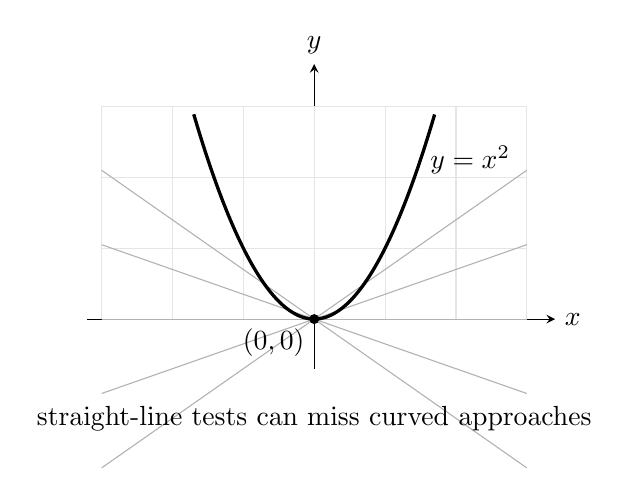
\begin{tikzpicture}[scale=0.9, >=stealth]
    \draw[->] (-3.2,0) -- (3.4,0) node[right] {\(x\)};
    \draw[->] (0,-0.7) -- (0,3.6) node[above] {\(y\)};

    \draw[gray!20, step=1] (-3,0) grid (3,3);

    \foreach \m in {-0.7,-0.35,0,0.35,0.7} {
        \draw[thin, gray!60] (-3,{-3*\m}) -- (3,{3*\m});
    }

    \draw[very thick, domain=-1.7:1.7, samples=80, smooth, variable=\x]
        plot ({\x},{\x*\x});
    \node[right] at (1.5,2.25) {\(y=x^2\)};

    \fill (0,0) circle (2pt);
    \node[below left] at (0,0) {\((0,0)\)};

    \node at (0,-1.4) {straight-line tests can miss curved approaches};
\end{tikzpicture}
\caption{All straight paths can agree while a curved path disagrees.}
\end{figure}

The moral is sharper now:

\[
    \text{Different path limits disprove a limit.}
\]
But
\[
    \text{matching path limits along many chosen paths do not prove a limit.}
\]

To prove a limit, we need a bound that controls all paths at once.

\subsection{Separate continuity does not imply continuity}

There is another tempting shortcut.  If a function is continuous in \(x\) when \(y\) is
held fixed, and continuous in \(y\) when \(x\) is held fixed, should it be continuous
as a function of both variables?

No.

Define
\[
    S(x,y)=
    \begin{cases}
    \dfrac{xy}{x^2+y^2}, & (x,y)\ne(0,0),\\[2mm]
    0, & (x,y)=(0,0).
    \end{cases}
\]

First hold \(y\) fixed.  If \(y=0\), then
\[
    S(x,0)=0,
\]
which is continuous in \(x\).  If \(y=y_0\ne0\), then
\[
    S(x,y_0)=\frac{xy_0}{x^2+y_0^2},
\]
which is a continuous function of \(x\).

So \(S\) is continuous in \(x\) when \(y\) is held fixed.

Similarly, holding \(x\) fixed gives a continuous function of \(y\).  The function is
continuous in each variable separately.

But as a two-variable function, \(S\) is not continuous at the origin.  Along the line
\(y=x\),
\[
    S(x,x)=\frac{x^2}{2x^2}=\frac12.
\]
Along the \(x\)-axis,
\[
    S(x,0)=0.
\]
So the limit at the origin does not exist.

This example will matter again in Chapter \ref{ch:7}.  Partial derivatives look at
coordinate directions.  Coordinate directions are important, but they are not the whole
plane.

\subsection{Why pictures can mislead near a singular point}

Graphs and contour maps are powerful, but they have a weakness: a very thin feature
can be invisible at normal scale.

Define
\[
    M(x,y)=
    \begin{cases}
    1, & 0<y<x^4,\\
    0, & \text{otherwise}.
    \end{cases}
\]
Near the origin, the region
\[
    0<y<x^4
\]
is a very thin strip above the \(x\)-axis.

Along any line
\[
    y=mx,
\]
the function eventually equals \(0\) near the origin.  To see why, suppose \(m\ne0\).
The condition
\[
    0<mx<x^4
\]
would imply, for small nonzero \(x\),
\[
    0<m<x^3
\]
or a similar impossible inequality after choosing the sign of \(x\).  For sufficiently
small \(x\), no fixed nonzero slope can fit inside the narrow strip.  The line \(y=0\)
also gives \(M=0\).

So every straight-line test gives the value \(0\).

But along the curve
\[
    y=\frac{x^4}{2},
\]
we have
\[
    0<\frac{x^4}{2}<x^4
\]
for every \(x\ne0\).  Therefore
\[
    M\left(x,\frac{x^4}{2}\right)=1.
\]
This curved path approaches the origin while the function stays equal to \(1\).  Hence
the limit at the origin does not exist.

\begin{figure}[h]
\centering
\begin{tikzpicture}[scale=2.2, >=stealth]
    \draw[->] (-1.35,0) -- (1.45,0) node[right] {\(x\)};
    \draw[->] (0,-0.08) -- (0,1.05) node[above] {\(y\)};

    \path[fill=gray!25]
        plot[domain=-1:1, samples=120, smooth, variable=\x]
        ({\x},{\x*\x*\x*\x})
        -- (1,0) -- (-1,0) -- cycle;

    \draw[thick, domain=-1:1, samples=120, smooth, variable=\x]
        plot ({\x},{\x*\x*\x*\x});
    \node[right] at (1,1) {\(y=x^4\)};

    \draw[dashed, thick, domain=-1:1, samples=120, smooth, variable=\x]
        plot ({\x},{0.5*\x*\x*\x*\x});
    \node[right] at (0.85,0.26) {\(y=\dfrac{x^4}{2}\)};

    \node at (0.1,0.12) {\(M=1\)};
    \node[below] at (0.65,0) {\(M=0\) on \(y=0\)};

    \fill (0,0) circle (0.8pt);
\end{tikzpicture}
\caption{A thin curved strip can be missed by every straight-line test.}
\end{figure}

This is the geometric reason line tests are dangerous.  A line is only one kind of road.
A function can hide its bad behavior between all the straight roads.

The chapter began with functions as fields of values.  It ends with a warning: fields can
be subtle near a point.  The next chapter asks a new question.  When a scalar field is
continuous enough to behave well, how fast is it changing?  In one variable there was
one derivative.  On a surface, there are many possible directions to move, so the word
``slope'' has to split into several ideas.

\section{Chapter review and discovery problems}
\label{sec:6.6}

This chapter changed the shape of calculus.  A function no longer has to take one
number as input.  Its input may be a point in the plane or in space, and its output may
be a number or a vector.

The new difficulty was not the algebra.  It was approach.  In one variable, a limit only
had to survive left and right.  In several variables, it must survive every path.

\subsection*{Chapter map}

\[
\begin{array}{c|p{8.5cm}}
\text{Idea} & \text{What it means} \\ \hline
F:\mathbb R^n\to\mathbb R^m
&
A function with \(n\) input coordinates and \(m\) output coordinates.\\[1mm]
\text{scalar field}
&
A function whose output is one number, such as temperature or height.\\[1mm]
\text{vector field}
&
A function whose output is a vector, such as wind velocity or force.\\[1mm]
\text{graph } z=f(x,y)
&
A surface made by placing height \(f(x,y)\) above each input point.\\[1mm]
\text{level curve}
&
A set \(f(x,y)=c\), showing where a scalar field has one fixed value.\\[1mm]
\text{level surface}
&
A set \(f(x,y,z)=c\), the three-dimensional version of a contour line.\\[1mm]
\text{limit}
&
The value a function approaches as the input approaches a point from every path.\\[1mm]
\text{continuity}
&
The function's actual value agrees with the value forced by nearby inputs.
\end{array}
\]

\subsection*{Concept checks}

\begin{enumerate}
\item Explain the difference between a scalar field and a vector field.  Give one
physical example of each.

\item A function has notation
\[
    F:\mathbb R^2\to\mathbb R^3.
\]
What is the shape of its input?  What is the shape of its output?

\item Why is the domain part of the meaning of a function, not just a technical detail?

\item Explain how a level curve of \(f(x,y)\) is related to a horizontal slice of the graph
\(z=f(x,y)\).

\item Can two level curves of the same function with different level values cross?
Explain.

\item Why can checking the \(x\)-axis and \(y\)-axis be enough to disprove a limit, but
not enough to prove one?

\item What does polar coordinates change about a limit near the origin?

\item State the three things that must be true for \(f\) to be continuous at a point
\(\mathbf a\).

\item Why does the Extreme Value Theorem require the domain to be closed and
bounded?

\item Give an example of a function that has a limit at a point but is not continuous
there.
\end{enumerate}

\subsection*{Skills: domains}

Find the natural domain of each function.  Describe the domain in words or with a
sketch when possible.

\begin{enumerate}
\item
\[
    f(x,y)=\sqrt{9-x^2-y^2}.
\]

\item
\[
    g(x,y)=\ln(4-x^2-y^2).
\]

\item
\[
    h(x,y,z)=\frac{1}{z^2-x^2-y^2}.
\]

\item
\[
    \mathbf F(x,y)=\bigl(\sqrt{x-y},\ln(x+y)\bigr).
\]

\item
\[
    p(x,y,z)=\frac{\sqrt z}{1-x^2-y^2}.
\]

\item
\[
    q(x,y)=\frac{1}{\sqrt{x^2+y^2-1}}.
\]
\end{enumerate}

\subsection*{Skills: graphs, level curves, and level surfaces}

\begin{enumerate}
\setcounter{enumi}{6}

\item Let
\[
    f(x,y)=4-x-y.
\]
Find the level curves \(f(x,y)=0,1,2,3\).  What kind of surface is the graph
\(z=f(x,y)\)?

\item Let
\[
    H(x,y)=100-x^2-9y^2.
\]
Find the level curves
\[
    H=99,\qquad H=91,\qquad H=64.
\]
Which direction is steeper, the \(x\)-direction or the \(y\)-direction?

\item Let
\[
    R(x,y,z)=(x-2)^2+(y+1)^2+z^2.
\]
Describe the level surfaces \(R=1\), \(R=4\), and \(R=9\).

\item Describe the level surfaces
\[
    z^2-x^2-y^2=c
\]
for
\[
    c=0,\qquad c=1,\qquad c=-1.
\]

\item Let
\[
    f(x,y)=xy.
\]
Sketch the level curves
\[
    xy=-2,\quad xy=-1,\quad xy=0,\quad xy=1,\quad xy=2.
\]
What happens at the level \(0\)?

\item Let
\[
    f(x,y)=x^2+y^2.
\]
Explain why the level curves are circles.  What happens to the spacing between
the curves if the levels are
\[
    1,\quad 4,\quad 9,\quad 16?
\]
\end{enumerate}

\subsection*{Skills: limits}

Evaluate each limit or show that it does not exist.

\begin{enumerate}
\setcounter{enumi}{12}

\item
\[
    \lim_{(x,y)\to(0,0)}
    \frac{x^2+y^2}{1+x^2+y^2}.
\]

\item
\[
    \lim_{(x,y)\to(0,0)}
    \frac{x^3+y^3}{x^2+y^2}.
\]

\item
\[
    \lim_{(x,y)\to(0,0)}
    \frac{xy}{\sqrt{x^2+y^2}}.
\]

\item
\[
    \lim_{(x,y)\to(0,0)}
    \frac{x^2-y^2}{x^2+y^2}.
\]

\item
\[
    \lim_{(x,y)\to(0,0)}
    \frac{x+y}{x-y}.
\]

\item
\[
    \lim_{(x,y)\to(0,0)}
    \frac{x^2y}{x^4+y^2}.
\]

\item
\[
    \lim_{(x,y)\to(0,0)}
    \frac{x^2y^2}{x^2+y^2}.
\]

\item
\[
    \lim_{(x,y)\to(1,2)}
    \frac{x^2+y^2}{x+y}.
\]

\item
\[
    \lim_{(x,y,z)\to(0,0,0)}
    \frac{x^2+y^2+z^2}{\sqrt{x^2+y^2+z^2}+1}.
\]

\item Let
\[
    F(x,y)=
    \left(
        x+y,\,
        \frac{x^2y}{x^2+y^2}
    \right),
    \qquad (x,y)\ne(0,0).
\]
Find
\[
    \lim_{(x,y)\to(0,0)}F(x,y),
\]
if it exists.
\end{enumerate}

\subsection*{Skills: continuity}

\begin{enumerate}
\setcounter{enumi}{22}

\item Determine where the function
\[
    f(x,y)=\frac{\sqrt{x-y}}{x^2+y^2-4}
\]
is continuous.

\item Define
\[
    f(x,y)=
    \begin{cases}
    \dfrac{x^2y}{x^2+y^2}, & (x,y)\ne(0,0),\\[2mm]
    k, & (x,y)=(0,0).
    \end{cases}
\]
Find the value of \(k\) that makes \(f\) continuous at the origin.

\item Define
\[
    g(x,y)=
    \begin{cases}
    \dfrac{xy}{x^2+y^2}, & (x,y)\ne(0,0),\\[2mm]
    k, & (x,y)=(0,0).
    \end{cases}
\]
Show that no value of \(k\) makes \(g\) continuous at the origin.

\item Let
\[
    f(x,y)=\ln(9-x^2-y^2),
\]
and let
\[
    \Phi(r,\theta)=(r\cos\theta,r\sin\theta).
\]
Find
\[
    (f\circ\Phi)(r,\theta)
\]
and describe where it is continuous.

\item Let
\[
    D=\{(x,y):x\ge0,\ y\ge0,\ x+y\le1\}.
\]
Explain why every continuous function on \(D\) has an absolute maximum and an
absolute minimum.

\item For each domain below, say whether it is closed, bounded, both, or neither:
\[
    x^2+y^2<1,
\]
\[
    x^2+y^2\le1,
\]
\[
    y\ge x^2,
\]
\[
    0<x<1,\quad 0<y<1.
\]
\end{enumerate}

\subsection*{Discovery problems}

\begin{enumerate}
\setcounter{enumi}{28}

\item \textbf{A contour map from a table.}
The table below gives measured temperatures, in degrees Celsius, on a square plate.
The row label is \(y\), and the column label is \(x\).

\[
\begin{array}{c|ccccc}
y\backslash x & 0 & 1 & 2 & 3 & 4 \\ \hline
4 & 18 & 19 & 20 & 19 & 18\\
3 & 19 & 21 & 24 & 21 & 19\\
2 & 20 & 24 & 30 & 24 & 20\\
1 & 19 & 21 & 24 & 21 & 19\\
0 & 18 & 19 & 20 & 19 & 18
\end{array}
\]

Draw an approximate contour map for the levels
\[
    20,\qquad 22,\qquad 24,\qquad 28.
\]
Where does the plate appear hottest?  Where are the contour lines closest together?

\item \textbf{A thin ridge.}
For
\[
    M(x,y)=
    \begin{cases}
    1, & 0<y<x^4,\\
    0, & \text{otherwise},
    \end{cases}
\]
show that every straight-line path through the origin gives limiting value \(0\),
but the path
\[
    y=\frac{x^4}{2}
\]
gives limiting value \(1\).  Explain why a computer graph of \(M\) might miss the
problem near the origin.

\item \textbf{Invent your own path test.}
Find a function
\[
    f(x,y)
\]
whose limit at the origin fails because two parabolic paths give different limiting
values.  The two paths should not be straight lines.

\item \textbf{Repairing a discontinuity.}
Find a function \(f(x,y)\) that is not defined at the origin but has a limit there.
Then define a new function \(F\) by assigning one value at the origin so that \(F\)
becomes continuous at the origin.

\item \textbf{Real contour project.}
Choose a small real data set that depends on two variables.  Examples include
temperature on a tabletop, light intensity in a room, elevation on a hiking map, or
sound level at different locations.

Make a table of values, draw an approximate contour map, and write a paragraph
answering these questions:
\[
\begin{array}{l}
\text{Where is the quantity largest?}\\
\text{Where is it smallest?}\\
\text{Where does it seem to change fastest?}\\
\text{What features of the contour map tell you that?}
\end{array}
\]
\end{enumerate}

A contour map shows where a function has the same value.  Limits and continuity tell
us when those values settle down near a point.  But they do not yet tell us how fast the
values change.

On a hillside, we can walk east, north, northeast, or along any path we choose.  Each
direction may give a different slope.  The next chapter begins with the simplest version
of that idea: hold all variables still except one, and take an ordinary single-variable
derivative in that slice.  These are called \emph{partial derivatives}, and they are the
first step toward the full multivariable derivative.

